%!TEX root = ../main.tex
\newpage
\section{Evaluation on Field Data}\label{sec:eval_field}

本節では、\cref{chap:experiments}に従い宇治川中流域の副流\cref{sec:field-dataset}を対象に行なった、RA-GSの2DGSによる屈折を排した三次元再構成の結果に関して述べる。
最適化にはADCを用い、30k回のイテレーションで実施した。

\subsection{Qualitative Evaluation}\label{subsec:eval_field_qualitative}

\begin{figure}[htbp]
  \centering
  \begin{subfigure}[t]{\textwidth}
    \centering
    \includegraphics[height=8cm, keepaspectratio]{figure/80_eval/field/cray_wo.png}
    \caption{2DGS(補正無し)}
  \end{subfigure}

  \begin{subfigure}[t]{\textwidth}
    \centering
    \includegraphics[height=8cm, keepaspectratio]{figure/80_eval/field/cray_full.png}
    \caption{Ours}
  \end{subfigure}
  % --- 全体設定 ---
  \caption{
    2DGS(補正無し)とRA-GSによる再構成結果の比較。
    抽出されたメッシュをクレイレンダリングで表示している。
    RS-GSには位置、共分散、放射輝度補正を適用している。
    RA-GSでは、より見かけの浅さを除外し、より深い位置に形状を復元している。
  }
  \label{fig:eval_field_cray}
\end{figure}

\ref{fig:eval_field_cray}に示すように、RA-GSによる再構成結果は、2DGS(補正無し)に比べて、より深い位置に形状を復元している。
これは、正確に屈折を考慮した補正が適用され、見かけの浅さの影響が除外できているからだと考えられる。

\begin{sidewaysfigure}[htbp]
  \centering 
  \captionsetup{justification=raggedright}
  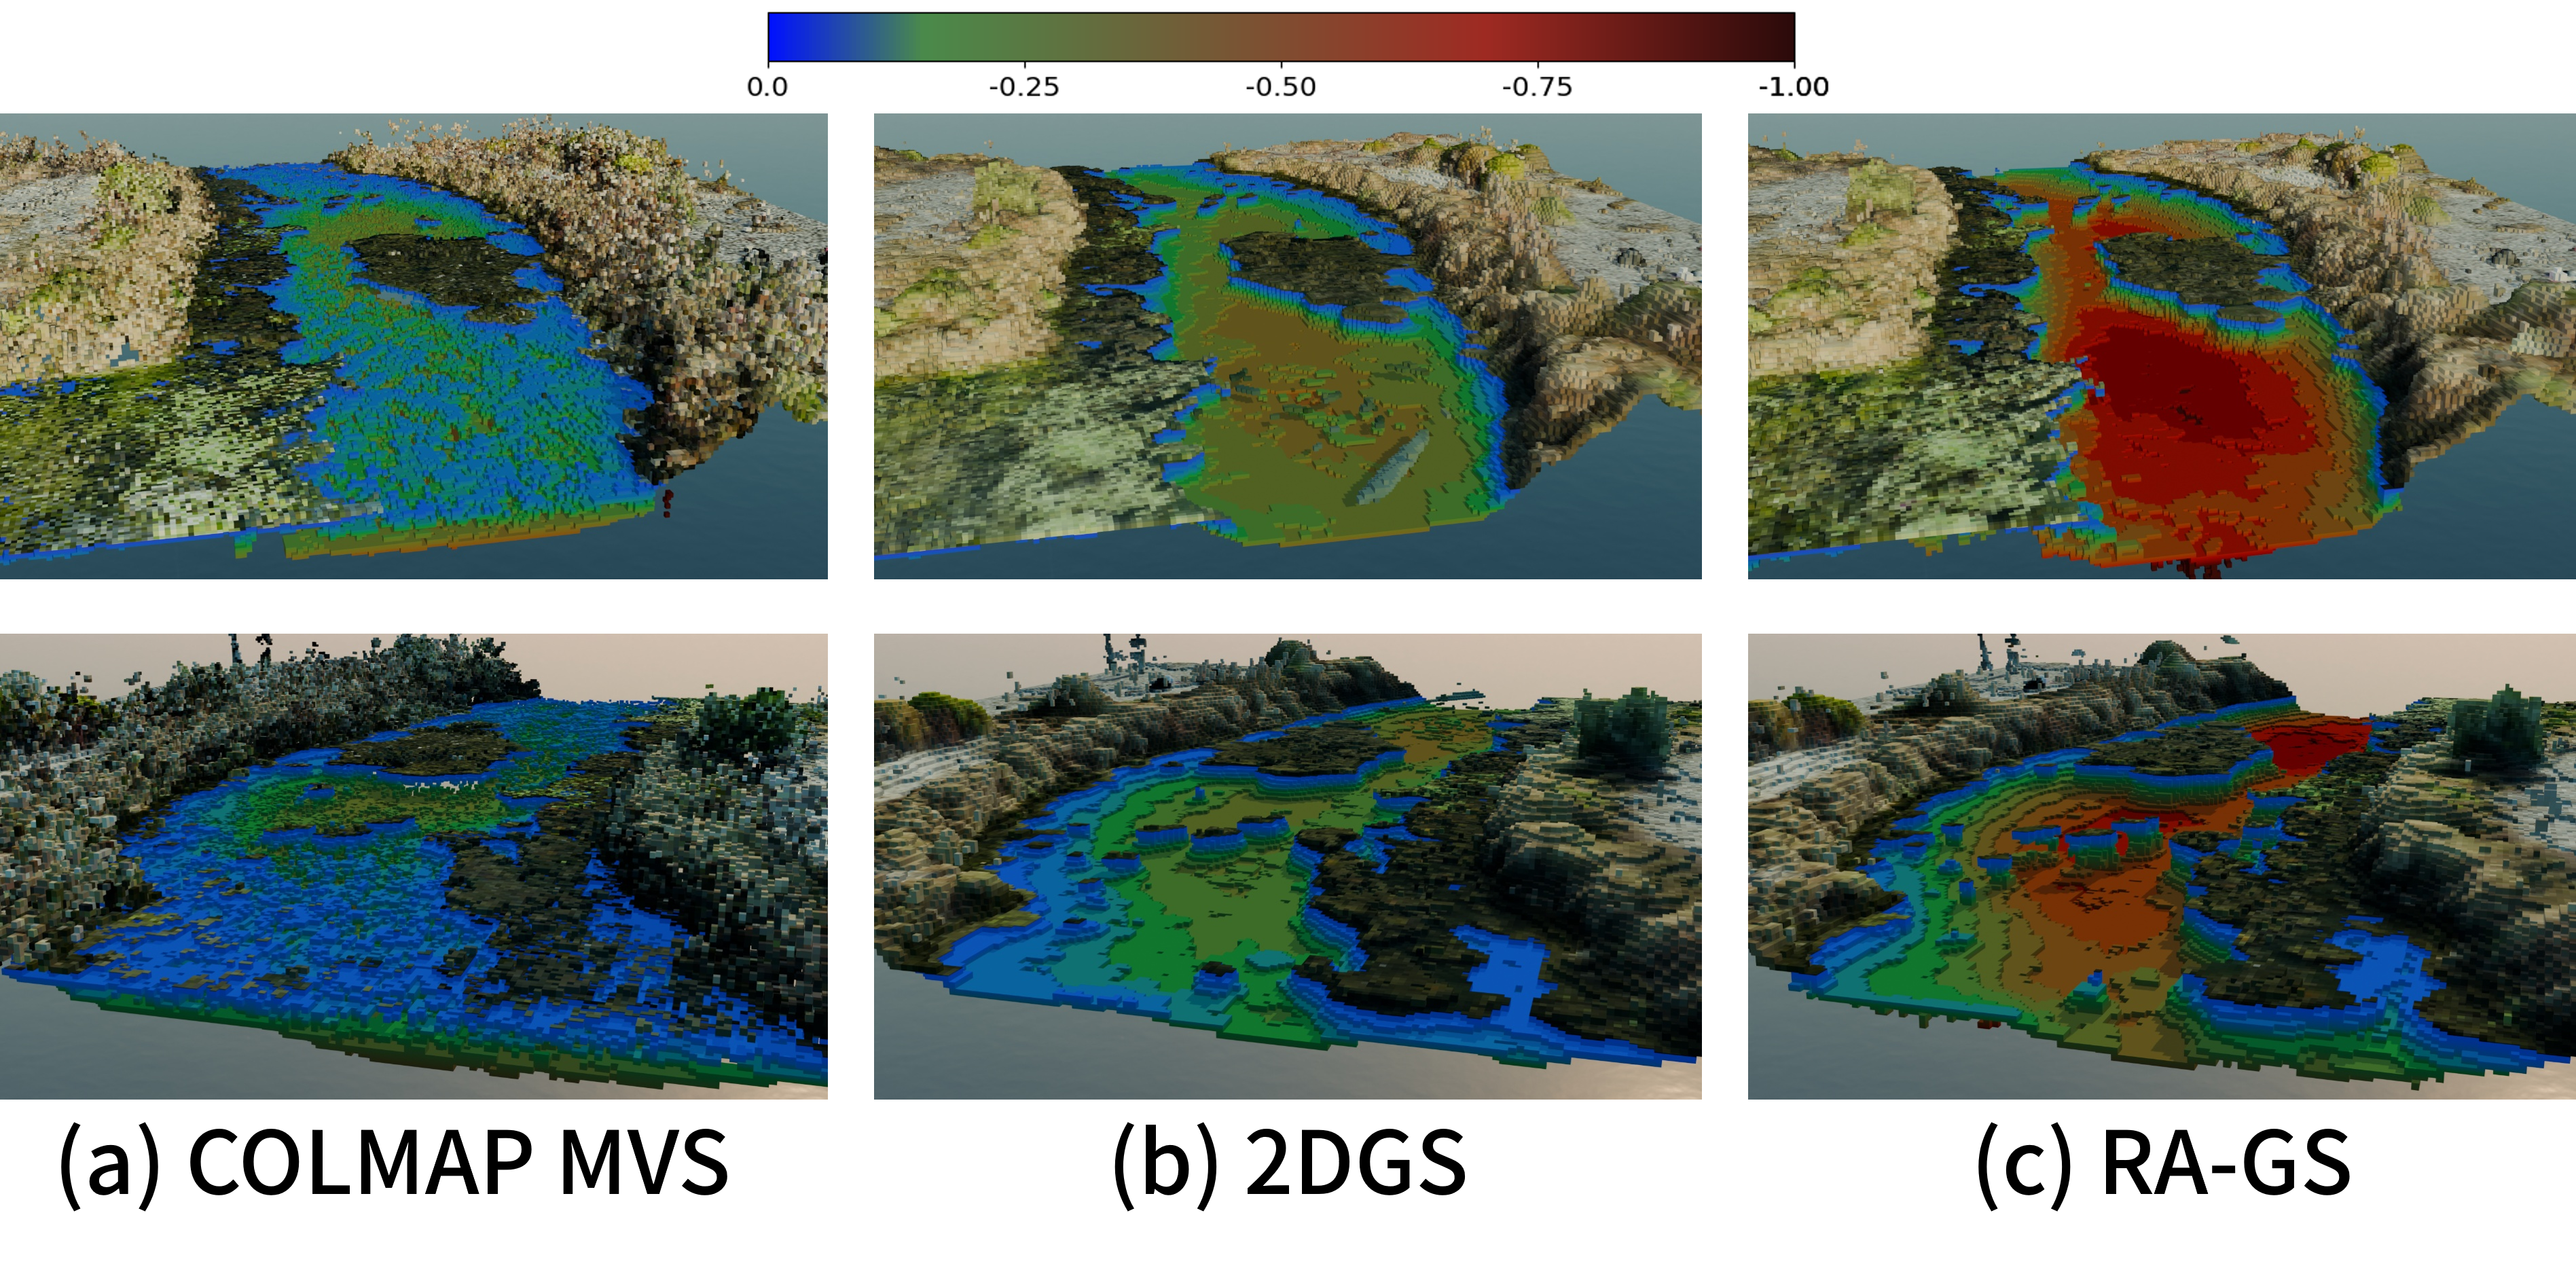
\includegraphics[width=0.95\textheight]{figure/80_eval/field/voxel-height.png}
  \caption{
    COLMAP MVS、2DGS、RA-GSによる深度の比較。
    形状が分かりやすいようにVoxel化し、深度が深くなるに連れ赤色に着色している。
    }
  \label{fig:eval_field_voxel_height}
\end{sidewaysfigure}

\ref{fig:eval_field_voxel_height}は、COLMAPによるMVS実装\cite{Schonberger2016ECCV_PatchMatchStereo}を比較に加え、深度を色で明示している。
形状が分かりやすいように各構成結果を0.08 cm単位のボクセル(Voxel)で区切り、水面下の形状を深度が深くになるにつれて青色から赤色にかけてのカラーランプで表示している。


